\subsection{Spoked Runner with Massless Legs}
\subsubsection*{System Setup}
\begin{itemize}

\item $m=15 $, $I_{yy} = 10$,  $l=4$,  $r_{penetration} = 0.3$ (the distance the virtual wheel penetrate into the ground)
\item Adjustable spoke leg number
\item Fixed rotation rate w.r.t inertial frame
\item Setup of contact force: PD control
\begin{itemize}
\item w.r.t to world frame
\item w.r.t to inertial frame (virtual pivot point)
\end{itemize}
\item Assuming no friction (Could be an bad idea?)
%\end{align*}
\end{itemize}
\begin{figure}[H]
\begin{subfigure}{.5\textwidth}
  \centering
  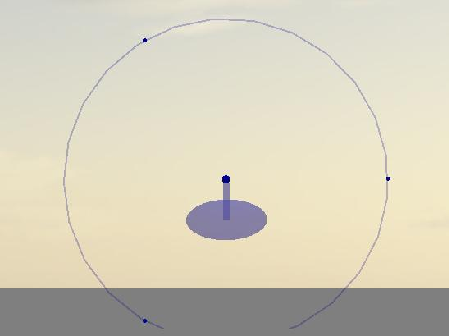
\includegraphics[width=.8\linewidth]{spokedRunner02.pdf}
  %\caption{1a}
  %\label{fig:sfig1}
\end{subfigure}%
\begin{subfigure}{.5\textwidth}
  \centering
  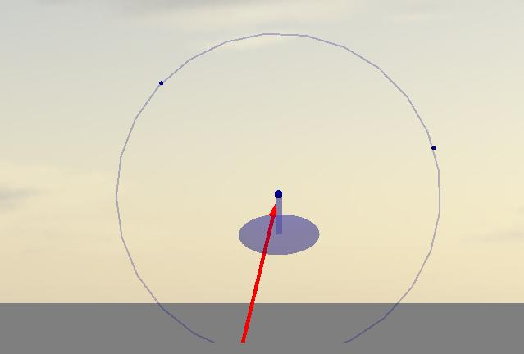
\includegraphics[width=.8\linewidth]{spokedRunner01.pdf}
  %\caption{1b}
  % \label{fig:sfig2}
\end{subfigure}
\caption{The Spoked Runner with three legs}
\label{fig:spokedRunner}
\end{figure}

\subsubsection*{Plan}

\begin{itemize}
\item Smoothly change the leg length, or the rotational speed of the virtual wheel, and observe the system response.
\item Learn how to use GUI for parameter adjustment with SCS.
\end{itemize}

%\begin{figure}[H]
%\centering
%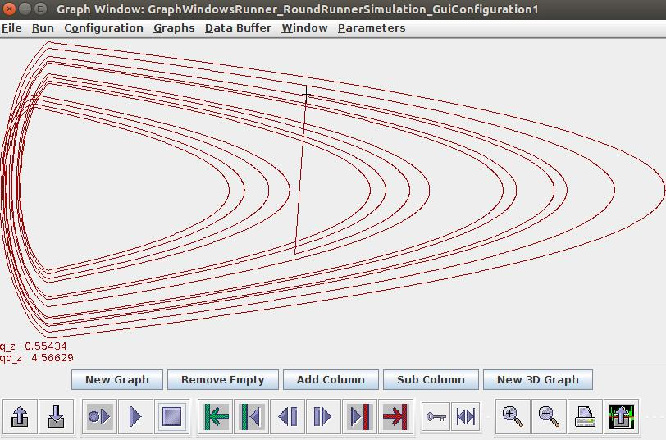
\includegraphics[scale = 0.8]{f100_unstable.pdf} 
%\caption{Phase portrait of $f = 100$ N, no stable limit cycle evolved (might be bifurcation).}
%%\label{fig.verticalHopper1DOF}
%\end{figure}